\documentclass[10pt,a4paper]{article}
\usepackage[T1]{fontenc}
\usepackage[utf8]{inputenc}
\usepackage{enumitem}
\usepackage{graphicx}
\usepackage{tabularx}
\usepackage{multirow}
\usepackage{helvet}
\usepackage{verbatim}
\usepackage[pdfborderstyle={/S/U/W 1}]{hyperref}
\usepackage[a4paper,margin=1in]{geometry}
\usepackage{float}
\usepackage[polish]{babel}

\renewcommand\familydefault{\sfdefault}

\begin{document}
\begin{titlepage}
	\centering
	{\Large Wydział Matematyki i Nauk Informacyjnych Politechniki Warszawskiej \par}
	\vspace{1cm}
	
\includegraphics[width=0.2\textwidth]{logo.png} \par
	\vspace{5cm}
	{\LARGE System informacji oraz sprzedaży biletów\\komunikacji miejskiej i międzymiastowej \par}
	\vspace{0.5cm}
	{\Large Bartłomiej Dach, Tymon Felski \par}
	\vspace{1.5cm}
	{\Large Wersja 1.0 \par}
	\vspace{1.5cm}
	{\Large \today \par}
\end{titlepage}
Lista zmian w dokumencie:
\begin{table}[H]
\def\arraystretch{1.5}
\begin{tabularx}{\textwidth}{|l|l|X|l|}
	\hline
	\textbf{Data} & \textbf{Autor} & \textbf{Opis zmian} & \textbf{Wersja} \\
	\hline
	16.10.2016 & Bartłomiej Dach, Tymon Felski & Określenie wymagań projektu oraz harmonogramu prac & 1.0 \\
	\hline
\end{tabularx}
\end{table}

\tableofcontents
\newpage

\section{Specyfikacja}

\subsection{Opis biznesowy}
Niniejszy system służy do przechowywania danych o przewoźnikach i połączeniach komunikacji miejskiej oraz międzymiastowej. Składowane dane wykorzystywane są do wyszukiwania konkretnych połączeń oraz sprzedaży biletów.

\subsection{Wymagania funkcjonalne}

\subsubsection*{Przypadki użycia}
Poniższy diagram UML przedstawia zbiór przypadków użycia aplikacji dla aktora -- pracownika firmy pośredniczącej w sprzedaży biletów wielu przewoźników.
\begin{figure}[H]
	\centering
	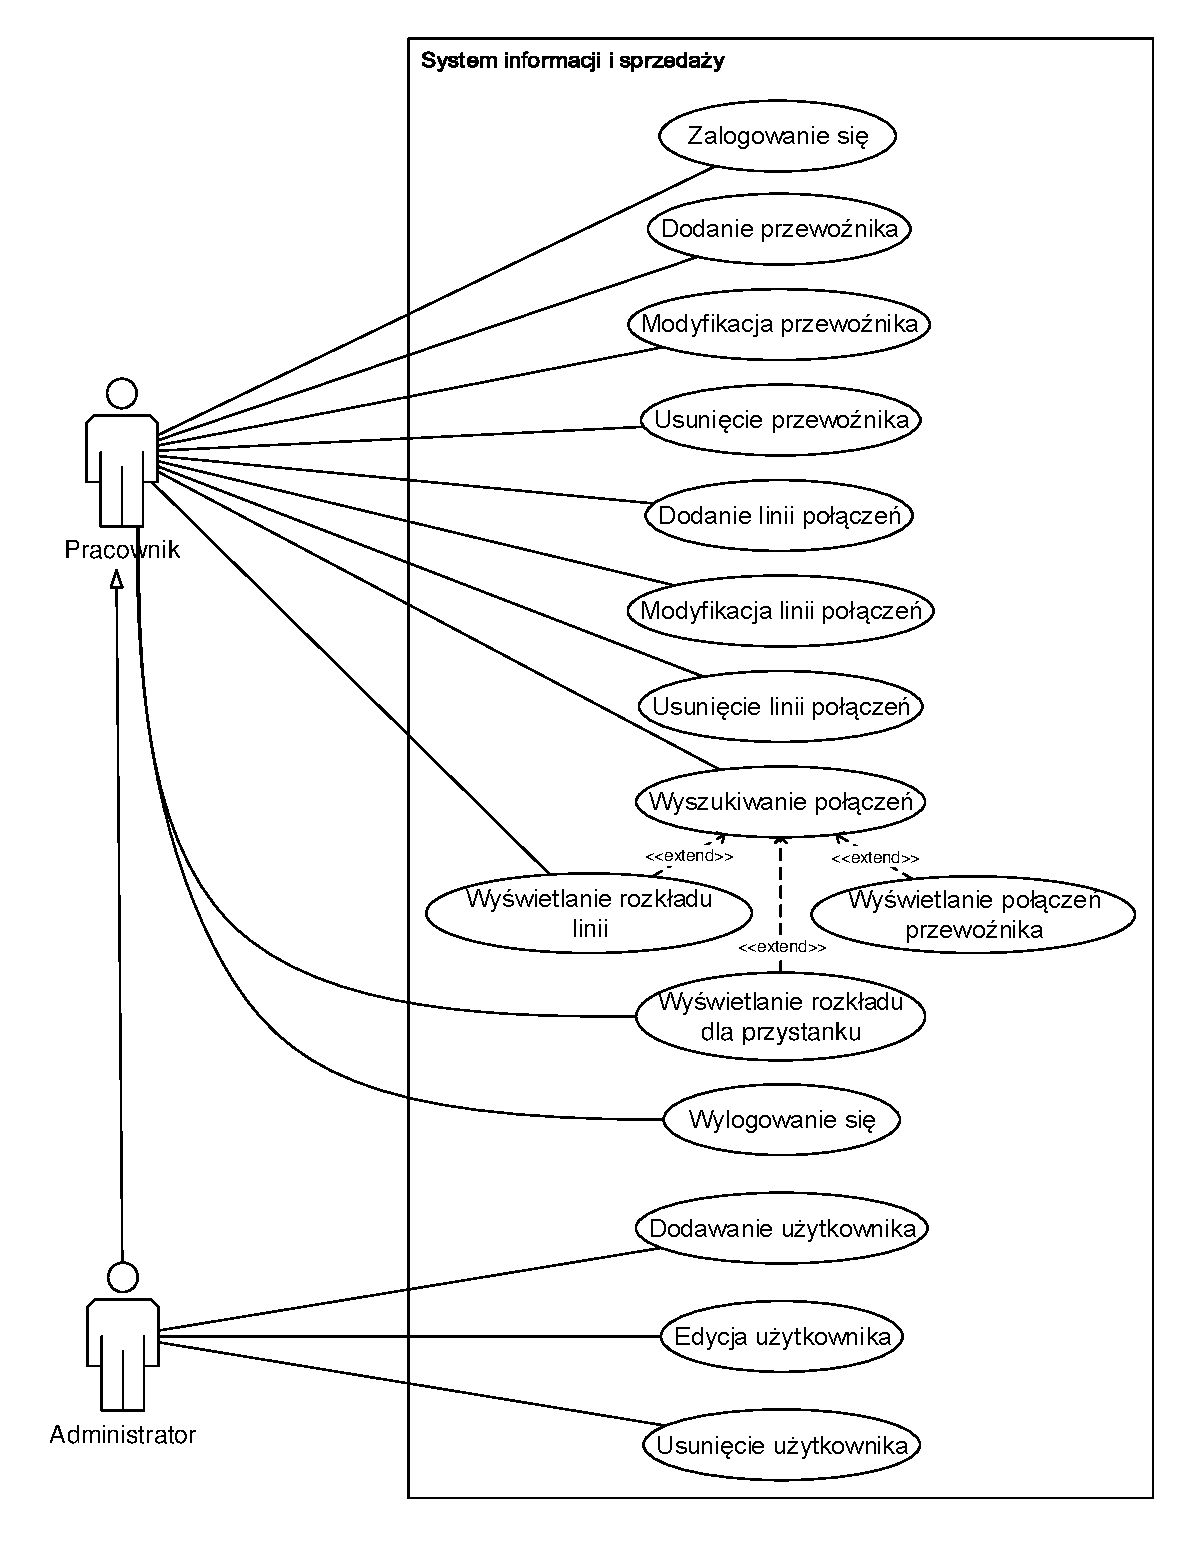
\includegraphics[width=12cm]{use-case.pdf}
	\caption{Diagram przypadków użycia dla aplikacji}
\end{figure}
Poszczególne przypadki są opisane szerzej w poniższej tabeli:
\begin{table}[H]
	\begin{tabularx}{\textwidth}{|c|X|X|X|}
		\hline
		\textbf{Aktor} & \textbf{Nazwa} & \textbf{Opis} & \textbf{Odpowiedź systemu} \\
		\hline
		\multirow{20}{*}{\rotatebox[origin=c]{90}{Pracownik}}
		& Zalogowanie się 
		& Zalogowanie się użytkownika do systemu
		& Potwierdzenie zalogowania się lub komunikat o błędzie \\
		\cline{2-4}
		& Dodanie przewoźnika
		& Dodanie informacji o nowym przewoźniku do bazy
		& Potwierdzenie dodania danych do bazy \\
		\cline{2-4}
		& Modyfikacja przewoźnika
		& Zmiana danych przewoźnika przechowywanych w bazie
		& Potwierdzenie zmodyfikowania rekordu \\
		\cline{2-4}
		& Dodanie linii połączeń
		& Dodanie nowej linii połączeń danego przewoźnika
		& Potwierdzenie dodania linii do bazy \\
		\cline{2-4}
		& Modyfikacja linii połączeń
		& Modyfikacja linii połączeń danego przewoźnika
		& Potwierdzenie modyfikacji rekordu \\
		\cline{2-4}
		& Wyszukiwanie połączeń
		& Wyszukiwanie połączeń przewoźników między wybranymi punktami
		& Widok z listą znalezionych połączeń \\
		\cline{2-4}
		& Wyświetlanie rozkładu
		& Wyświetlanie rozkładu jazdy wybranej linii
		& Widok zawierający informacje o przejazdach na wybranej linii \\
		\cline{2-4}
		& Wyświetlanie połączeń przewoźnika
		& Wyświetlanie połączeń obsługiwanych przez danego przewoźnika
		& Widok zawierający informacje o liniach danej firmy \\
		\cline{2-4}
		& Wylogowanie się
		& Wylogowanie się pracownika z systemu
		& Potwierdzenie zakończenia pracy z systemem \\
		\hline
	\end{tabularx}
	\caption{Opisy przypadków użycia dla użytkownika}
\end{table}

\subsubsection*{User stories}
\begin{enumerate}
	\bfseries
	\item Interfejs administracyjny dla pracownika
	\begin{enumerate}[label*=\arabic*.]
		\mdseries
		\item Jako zalogowany pracownik dodaję/modyfikuję przewoźnika. \\
			Dowolny zalogowany pracownik może dodać nowego przewoźnika lub zmodyfikować informacje o przewoźniku, takie, jak: nazwę i adres firmy, numer REGON, dane kontaktowe osoby odpowiadającej za współpracę w kwestii sprzedaży biletów.
		\item Jako zalogowany pracownik dodaję/modyfikuję linię połączeń. \\
			Dowolny zalogowany pracownik może dodać lub zmodyfikować informacje o nowym połączeniu takie jak: przystanki początkowe, pośrednie i końcowe, czas odjazdu i przyjazdu na poszczególnych przystankach, ilość dostępnych miejsc w danym kursie, podstawowa cena biletu oraz wysokość zniżek.
		\item Jako zalogowany pracownik wyświetlam rozkład jazdy dla wybranej linii. \\
		Dowolny zalogowany pracownik może wyświetlić rozkład jazdy wybranej linii. Z poziomu wyświetlania rozkładu pracownik może: dodać nowe połączenie tej linii, usunąć istniejące połączenie lub wygenerować rozkład jazdy w postaci pliku.
		\item Jako zalogowany pracownik wyszukuję połączenie. \\
		    Dowolny zalogowany pracownik może wyszukać dostępne połączenia pomiędzy
		    wprowadzonymi miastami.
	 	\item Jako zalogowany pracownik wyświetlam rozkład jazdy danej linii. \\
		    Dowolny zalogowany pracownik może wyszukać rozkład jazdy dla danej linii
		    komunikacyjnej i go wyświetlić.
	    	\item Jako zalogowany pracownik wyświetlam połączenia dla danego przewoźnika. \\
		    Dowolny zalogowany pracownik może wyświetlić połączenia od danego przewoźnika.
	\end{enumerate}
\end{enumerate}

\subsection{Wymagania niefunkcjonalne}
Poniższa tabela zawiera rozpisane wymagania niefunkcjonalne narzucone dla systemu.
\begin{table}[H]
	\begin{tabularx}{\textwidth}{|c|l|X|}
		\hline
		\textbf{Obszar wymagań} & \textbf{Nr} & \textbf{Opis} \\
		\hline
		\multirow{5}{*}{Użyteczność (\textit{Usability})}
		& 1 & Rozmiar czcionki użytej w aplikacji musi być nie mniejszy niż 12 punktów. \\
		\cline{2-3}
		& 2 & Aplikacja powinna obsługiwać zmianę rozmiaru okna w sposób który umożliwia korzystanie ze wszystkich jej funkcjonalności (tzw. responsive design). \\
		\hline
		\multirow{3}{*}{Niezawodność (\textit{Reliability})}
		& 3 & Aplikacja musi być odporna na dokonywanie jednoczesnych zmian tego samego rekordu bazy przez wielu pracowników jednocześnie. \\
		\hline
		\multirow{7}{*}{Wydajność (\textit{Performance})}
		& 4 & Aplikacja powinna dodawać nowe obiekty do systemu w czasie nie dłuższym niż 1 sekundę, przy 50 żądaniach dodania obiektu na minutę. \\
		\cline{2-3}
		& 5 & Zużycie pamięci RAM przez aplikację nie powinno przekroczyć 200 megabajtów. \\
		\cline{2-3}
		& 6 & Wyszukiwanie połączenia między określonymi miastami powinno trwać mniej niż 2 sekundy, przy ok. 10 tys. rekordów. \\
		\hline
		\multirow{2}{*}{Utrzymanie (\textit{Supportability})}
		& 7 & Do aplikacji dołączona zostanie instrukcja wykonywania kopii zapasowej danych. \\
		\hline
	\end{tabularx}
	\caption{Tabela wymagań niefunkcjonalnych}
\end{table}

\subsection{Harmonogram projektu}
Prace przy projekcie będą realizowane według następującego harmonogramu:
\begin{figure}[H]
	\centering
	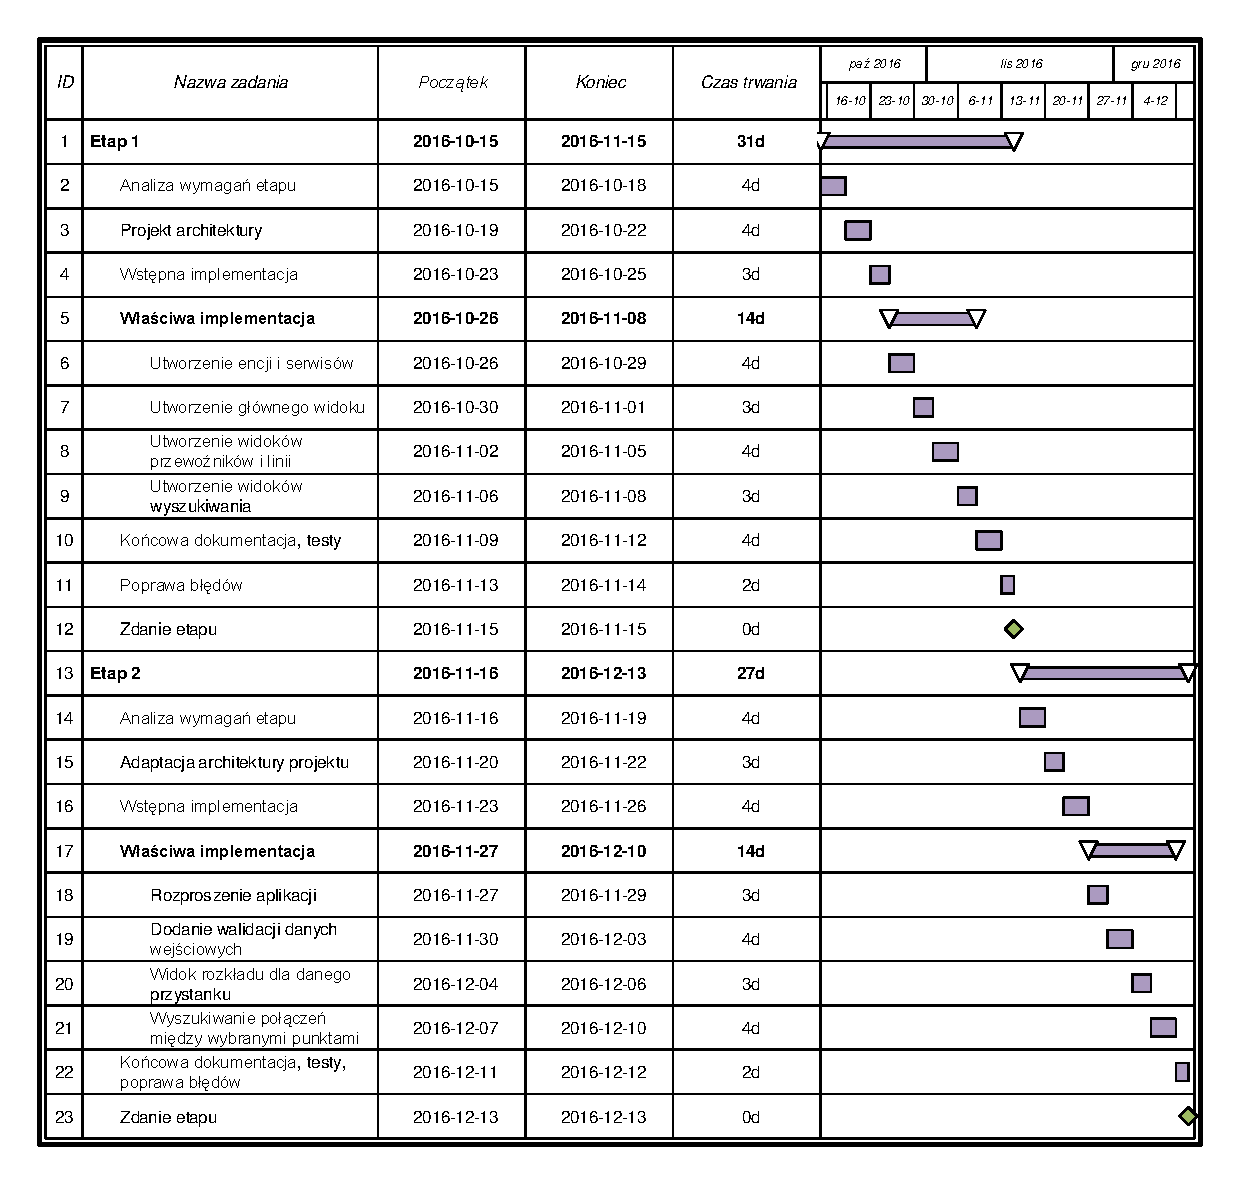
\includegraphics[width=16cm]{gantt.pdf}
	\caption{Diagram Gantta z planowanym harmonogramem projektu}
\end{figure}
Kamienie milowe:
\begin{enumerate}
	\item 18 października: Zakończenie analizy wymagań funkcjonalnych i niefunkcjonalnych projektu.
	\item 22 października: Zakończenie projektu architektury aplikacji, łącznie z wyróżnieniem komponentów oraz podsystemów.
	\item 25 października: Wstępna implementacja projektu architektury, naniesienie ewentualnych poprawek do architektury wynikających z problemów implementacyjnych.
	\item 29 października: Utworzenie encji biznesowych oraz serwisów wykorzystywanych przez użytkowników.
	\item 1 listopada: Utworzenie głównego widoku aplikacji.
	\item 5 listopada: Utworzenie widoków dodawania przewoźników oraz linii.
	\item 8 listopada: Utworzenie widoków wyszukiwania połączeń oraz wyświetlania połączeń danej linii oraz przewoźnika.
	\item 12 listopada: Zakończenie dokumentacji, testów aplikacji oraz identyfikacji błędów.
	\item 15 listopada: Zakończenie poprawy znalezionych błędów, zdanie projektu łącznie z pełną dokumentacją.
\end{enumerate}

\subsection{Architektura rozwiązania}
Docelowym środowiskiem aplikacji są małe lub średnie firmy pośredniczące w sprzedaży biletów komunikacyjnych, tzn. przedsiębiorstwa zatrudniające do 250 pracowników, z czego dostęp do systemu miałby dość niski procent tej liczby (w założeniach ok. 20-30\%). Dane, których przechowywanie jest niezbędne do spełnienia wymagań funkcjonalnych mają dość małą zmienność - stosunkowo rzadko ulegają zmianom lub przedawnieniom. Dodatkowo, ze względu na wewnętrzny charakter przechowywanych danych, system powinien być scentralizowany i znajdować się w jednym fizycznym położeniu.
\begin{figure}[H]
	\centering
	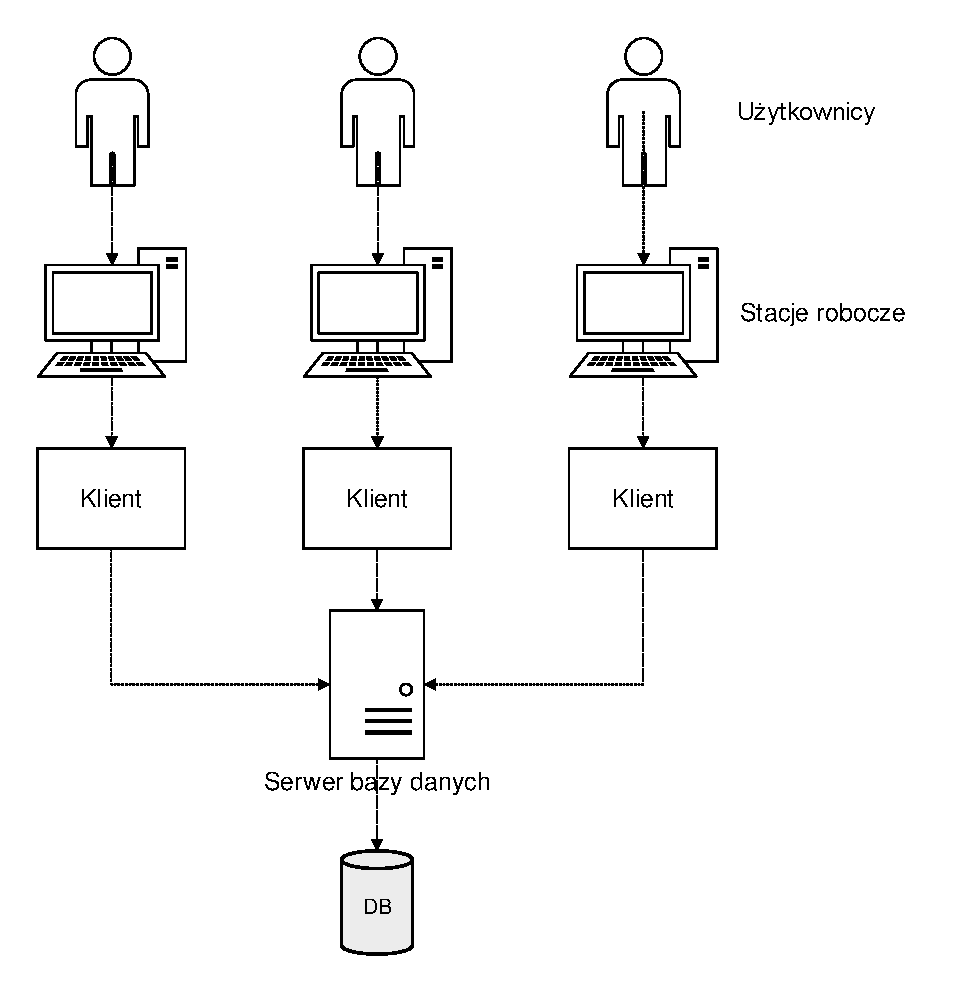
\includegraphics[width=10cm]{architecture-global.pdf}
	\caption{Schemat architektury systemu}
\end{figure}
Biorąc pod uwagę opisany powyżej charakter zamówionego rozwiązania, wybrana została prosta architektura z centralną bazą danych oraz aplikacją typu “gruby klient”, wykorzystującą bezpośrednie połączenie z bazą. Rozwiązanie to jest spójne z opisanymi cechami systemu, a poza tym jest dość proste we wdrożeniu i nie wprowadza niepotrzebnych kosztów rozproszenia.
\begin{figure}[H]
	\centering
	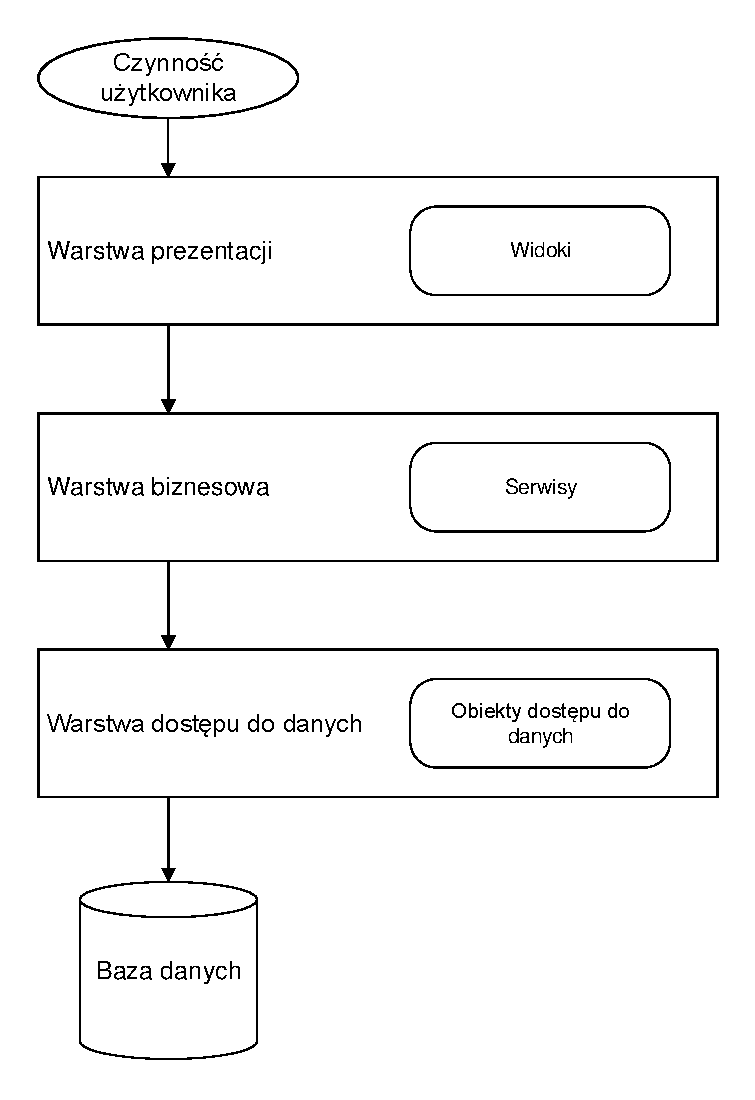
\includegraphics[width=8cm]{architecture-fat-client.pdf}
	\caption{Schemat architektury aplikacji klienckiej}
\end{figure}
Planowana architektura aplikacji klienckiej ma charakter warstwowy. Wyróżnione zostały następujące warstwy:
\begin{itemize}
\item warstwa dostępu do danych - odpowiedzialna za kontakt z bazą oraz odczyt i zapis przechowywanych tam danych,
\item warstwa biznesowa - odpowiedzialna za wykonywanie poszczególnych usług (np. dodania czy modyfikacji przewoźnika),
\item warstwa prezentacji - odpowiedzialna za wyświetlanie interfejsu użytkownika.
\end{itemize}
Głównymi powodami zaproponowania architektury warstwowej były:
\begin{itemize}
\item możliwość wymiany silnika bazodanowego oraz warstwy prezentacji bez naruszania warstwy biznesowej,
\item podział odpowiedzialności na poszczególne warstwy,
\item spójny charakter wymagań - podział na podsystemy jest zbędny.
\end{itemize}
Ze względu na małą liczbę użytkowników niska skalowalność oraz wydajność rozwiązań warstwowych zostały uznane za ryzyko drugorzędne.

\section{Dokumentacja końcowa (powykonawcza)}

\subsection{Wymagania systemowe}
% Punkt obowiązkowy.
%
% Rozdział powinien zawierać wymagania systemowe, wymagane oprogramowanie zewnętrzne
% (RDBMS, etc.)

\subsection{Biblioteki wraz z określeniem licencji}
W budowie aplikacji zostały użyte następujące biblioteki oraz komponenty firm trzecich:

\begin{table}[H]
	\begin{tabularx}{\textwidth}{|r|l|X|l|c|}
		\hline
		\textbf{Nr} & \textbf{Komponent i wersja} & \textbf{Opis} & \textbf{Licencja} & \\
		\hline
		1 & 
		Castle.Core, 3.3.3 &
		Wykorzystywana do tworzenia obiektów \textit{proxy}. Zależność biblioteki Moq. &
		Apache License 2.0 &
		\cite{castlecore} \\
		\hline
		2 &
		Entity Framework, 6.1.3 &
		Framework do mapowania obiektowo-relacyjnego (ORM). &
		Apache License 2.0 &
		\cite{entityframework} \\
		\hline
		3 &
		FluentAssertions, 4.17.0 &
		Wykorzystywany w testach jednostkowych w celu ułatwienia pisania asercji. &
		Apache License 2.0 &
		\cite{fluentassertions} \\
		\hline
		4 &
		Moq, 4.5.28 &
		Używany w testach jednostkowych do tworzenia obiektów zastępczych (tzw. \emph{mock object}). &
		\mbox{\hyperref[abbr:bsd]{BSD}} 3-Clause &
		\cite{moq} \\
		\hline
		5 &
		NUnit, 3.5.0 &
		Framework do wykonywania testów jednostkowych. &
		\mbox{\hyperref[abbr:mit]{MIT}} &
		\cite{nunit} \\
		\hline
		6 &
		ReactiveUI, 6.5.2 &
		Biblioteka wspomagająca w realizacji wzorca \hyperref[abbr:mvvm]{MVVM} w aplikacji klienckiej, zintegrowana z Reactive Extensions. &
		\mbox{\hyperref[abbr:mspl]{MS-PL}} &
		\cite{reactiveui} \\
		\hline
		7 &
		Reactive Extensions, 2.2.5 &
		Biblioteka wspomagająca w programowaniu aplikacji opartych na asynchronicznym przetwarzaniu danych oraz zdarzeniach. Zależność ReactiveUI. &
		Apache License 2.0 &
		\cite{reactiveextensions} \\
		\hline
		8 &
		Splat, 2.0.0 &
		Kontener \hyperref[abbr:IoC]{IoC} wspomagający w realizacji wzorca wstrzykiwania zależności. &
		\mbox{\hyperref[abbr:mit]{MIT}} &
		\cite{splat} \\
		\hline
	\end{tabularx}
	\caption{Lista użytych bibliotek i komponentów}
\end{table}

\subsection{Instrukcja instalacji}
% Punkt obowiązkowy.
%
% Niniejszy rozdział powinien kompletną instrukcję instalacji systemu/aplikacji umożliwiająca osobie
% oceniającej implementację danego rozwiązania. Uwaga: instrukcja powinna być dostoswana do
% instalacji na czystym systemie operacyjnym.

\subsection{Instrukcja uruchomienia}
% Punkt obowiązkowy.
% 
% Niniejszy rozdział powinien zawierać kompletną instrukcję uruchomienia systemu/aplikacji
% umożliwiającą osobie oceniającej weryfikację poprawności działania systemu.

\subsection{Instrukcja użycia}
% Punkt obowiązkowy.
%
% Niniejszy rozdział powinien zawierać kompletną instrukcję użycia (manual) systemu/aplikacji
% umożliwiająca osobie oceniającej weryfikację poprawności działania systemu.

\subsection{Instrukcja utrzymania}
% Punkt obowiązkowy.
%
% Niniejszy rozdział powinien zawierać kompletną instrukcję utrzymania systemu obejmującą procedury
% włączenia, wyłączenia systemu oraz procedury backup/restore.

\subsection{Raport odstępstw od specyfikacji wymagań}
% Punkt obowiązkowy.

\subsection{Dokumentacja usług Web Services}
% Punkt obowiązkowy
%
% Niniejszy rozdział powinien w przypadku, gdy system udostępnia publiczne usługi web services
% powinien zawierać dokumentację usług zamieszczone w formie opisowej lub np. wg specyfikacji
% swagger.

\section{Dokumentacja końcowa (powykonawcza) -- punkty wymagane przez prowadzącego zajęcia}

\subsection{Pseudokod}

\subsection{Diagramy sekwencji}
% Punkt obowiązkowy
%
% W przypadku projektów półsemestralnych lub dłuższych: w przypadku, gdy system składa się z
% komponentów rozproszonych należy dołączyć diagram(y) sekwencji. Rozdział zawierać powinien
% zawierać diagramy sekwencji opisujące komunikację pomiędzy systemami lub komponentami
% systemu. Należy w nim uwzględnić wszystkie przepływy komunikatów pomiędzy komponentami
% systemu lub systemami.

\subsection{Model danych}
% W przypadku projektów półsemestralnych lub dłuższych, gdy system składuje dane, należy opisać
% model danych. Model danych powinien być wyrażony przez diagram entity relationship w przypadku
% relacyjnej bazy danych. Zalecane jest wówczas opisanie znaczenia poszczególnych relacji, jak
% również czytelne oznaczenie rodzaju relacji (np. jeden do wielu) oraz kluczy głównych i kluczy obcych.
% W przypadku wykorzystania platform nierelacyjnych np. platform NoSQL lub składowania danych w
% plikach Apache Hadoop należy przedstawić opis konwencji zapisu danych. Jest to szczególnie istotne,
% gdy model danych jest prowadzony w trybie tzw. schema-on-read tzn. nie jest egzekwowany przez
% platformę składowania danych, a zależy wyłącznie od konwencji stosowanej przez aplikację np.
% konwencji nazewnictwa kolumn, treści wpisów w formacie JSON lub formatu sekwencji plików
% tworzonych w systemie plików HDFS.

\subsection{Scenariusz testów akceptacyjnych}
% W przypadku projektów półsemestralnych np. realizowanych w ramach projektu zespołowego.
% Rozdział powinien zawierać scenariusze testów akceptacyjnych nawiązujących do wymagań
% funkcjonalnych i niefunkcjonalnych systemu.

\subsection{Raport z przeprowadzonych testów}
% W przypadku projektów półsemestralnych np. realizowanych w ramach projektu zespołowego.
% Rozdział powinien zawierać scenariusze testów akceptacyjnych nawiązujących do wymagań
% funkcjonalnych i niefunkcjonalnych systemu i wyniki ich przeprowadzenia.

\section{Lista użytych skrótów}
\label{abbr:bsd}
\paragraph{BSD} Berkeley Software Distribution

\label{abbr:mit}
\paragraph{MIT} Massachussetts Institute of Technology  

\label{abbr:mspl}
\paragraph{MS-PL} Microsoft Software Public License

\label{abbr:mvvm}
\paragraph{MVVM} \emph{ang.} Model-View-ViewModel -- wzorzec używany w projektach realizowanych w technologii \hyperref[abbr:wpf]{WPF} pozwalający na odseparowanie logiki aplikacji od warstwy prezentacyjnej. 

\label{abbr:wpf}
\paragraph{WPF} Windows Presentation Framework

\renewcommand*{\refname}{\vspace*{-2em}}
\section{Bibliografia}
\begin{thebibliography}{99}

\bibitem{castlecore}
	Castle Project,
	\emph{Castle Core},
	\url{https://github.com/castleproject/Core}

\bibitem{entityframework}
	ASP.NET,
	\emph{Entity Framework 6},
	\url{https://github.com/aspnet/EntityFramework6}

\bibitem{fluentassertions}
	Dennis Doomen,
	\emph{FluentAssertions},
	\url{https://github.com/dennisdoomen/fluentassertions}

\bibitem{moq}
	Moq,
	\emph{Moq 4},
	\url{https://github.com/moq/moq4}

\bibitem{nunit}
	NUnit,
	\emph{NUnit},
	\url{https://github.com/nunit/nunit}

\bibitem{reactiveui}
	ReactiveUI,
	\emph{ReactiveUI},
	\url{https://github.com/reactiveui/ReactiveUI}

\bibitem{reactiveextensions}
	Reactive Extensions,
	\emph{Rx.NET},
	\url{https://github.com/Reactive-Extensions/Rx.NET}

\bibitem{splat}
	Paul Betts,
	\emph{Splat},
	\url{https://github.com/paulcbetts/splat}

\end{thebibliography}
\end{document}
